\begin{frame}
	\frametitle{$C_{2}$: Fuzzy Reasoning Framework for Video Indexing}
	 {\small
	\begin{itemize}
	 
% 	  \item $C_{2}$ : An \alert{automated} framework to \alert{construct} an ontology,
 	  \item Ontology Management: \textbf{\alert{Knowledge Extraction}}, 
 	  \textbf{\alert{Ontology Structure}}, \textbf{\alert{Reasoning}} and \textbf{\alert{Evolving}}.
	\end{itemize}
	}
	\begin{center}\hspace*{-1cm} 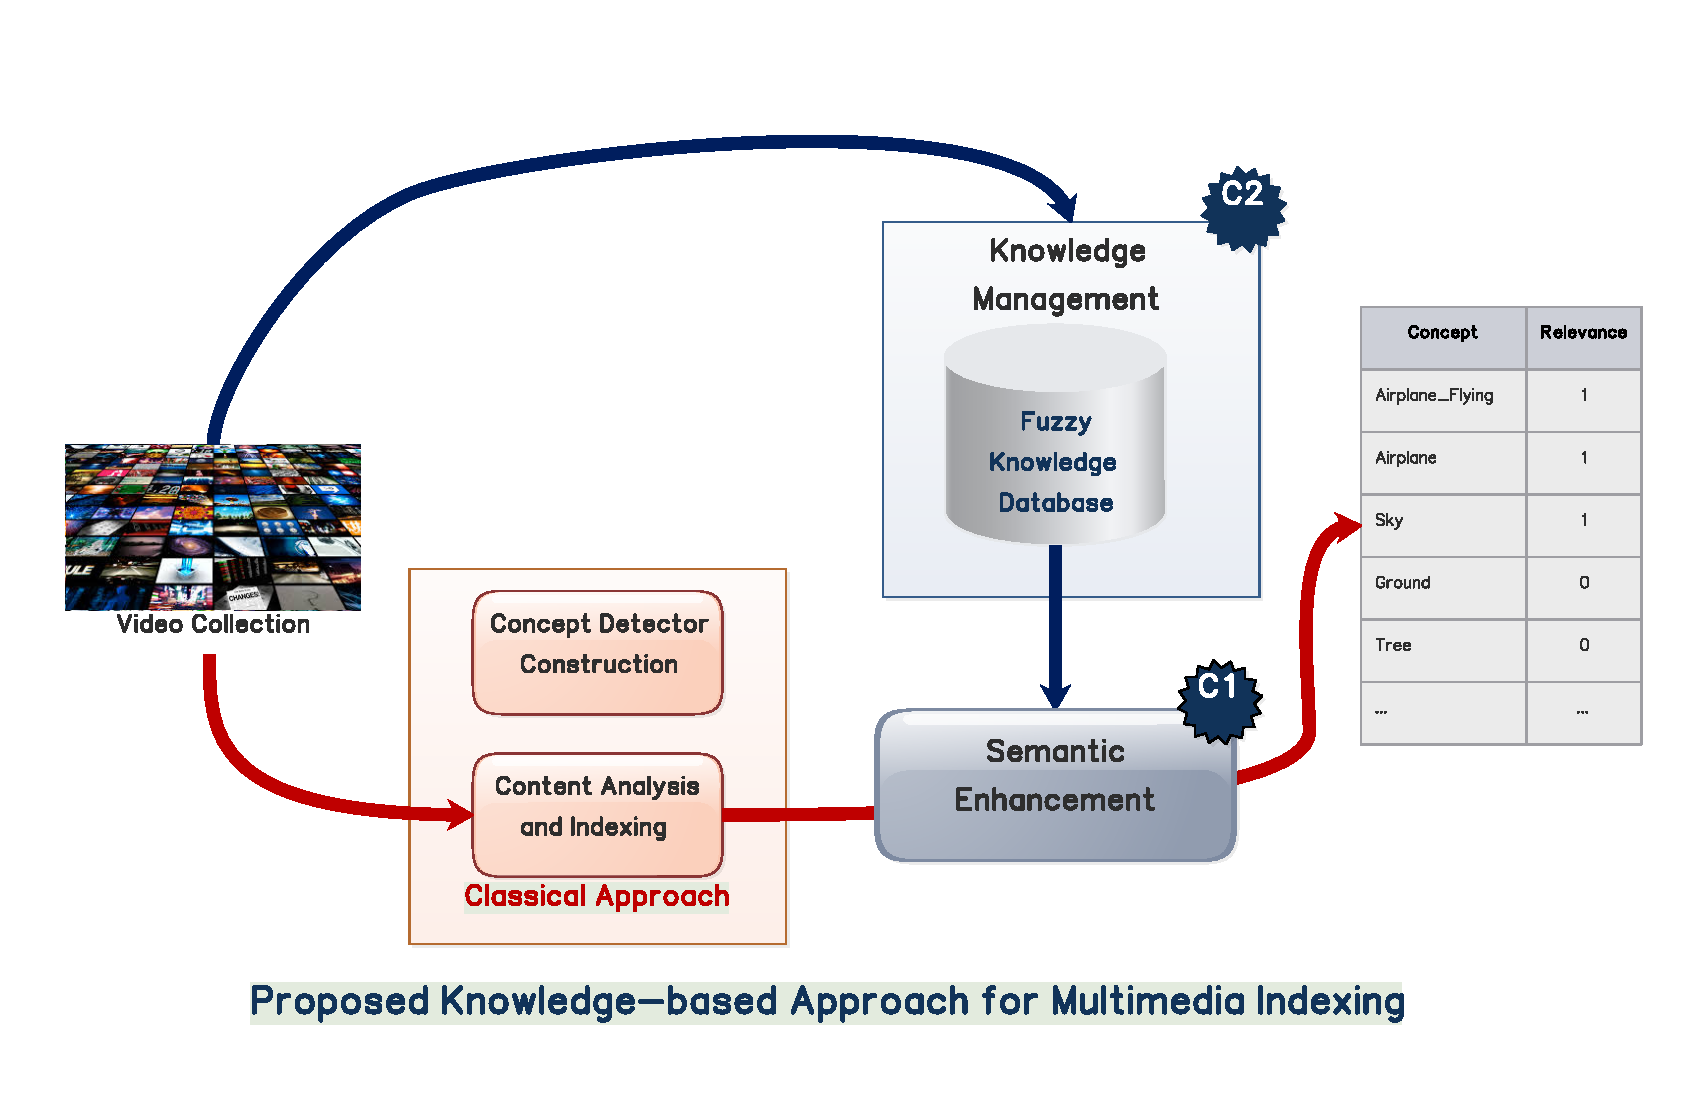
\includegraphics[scale=0.30]{graphics/contribution/contrib_overview_3} \end{center}

\end{frame}

\begin{frame}
	\frametitle{$C_{2}$: Proposed Approach - Inputs}
	\begin{block}{}
	 \begin{itemize}
	  \item \alert{Annotated} Multimedia Content,
	  \item A \alert{content} with a set of detected semantic \alert{concepts}.
	 \end{itemize}
	\end{block}

	{\hspace*{-1cm}\centering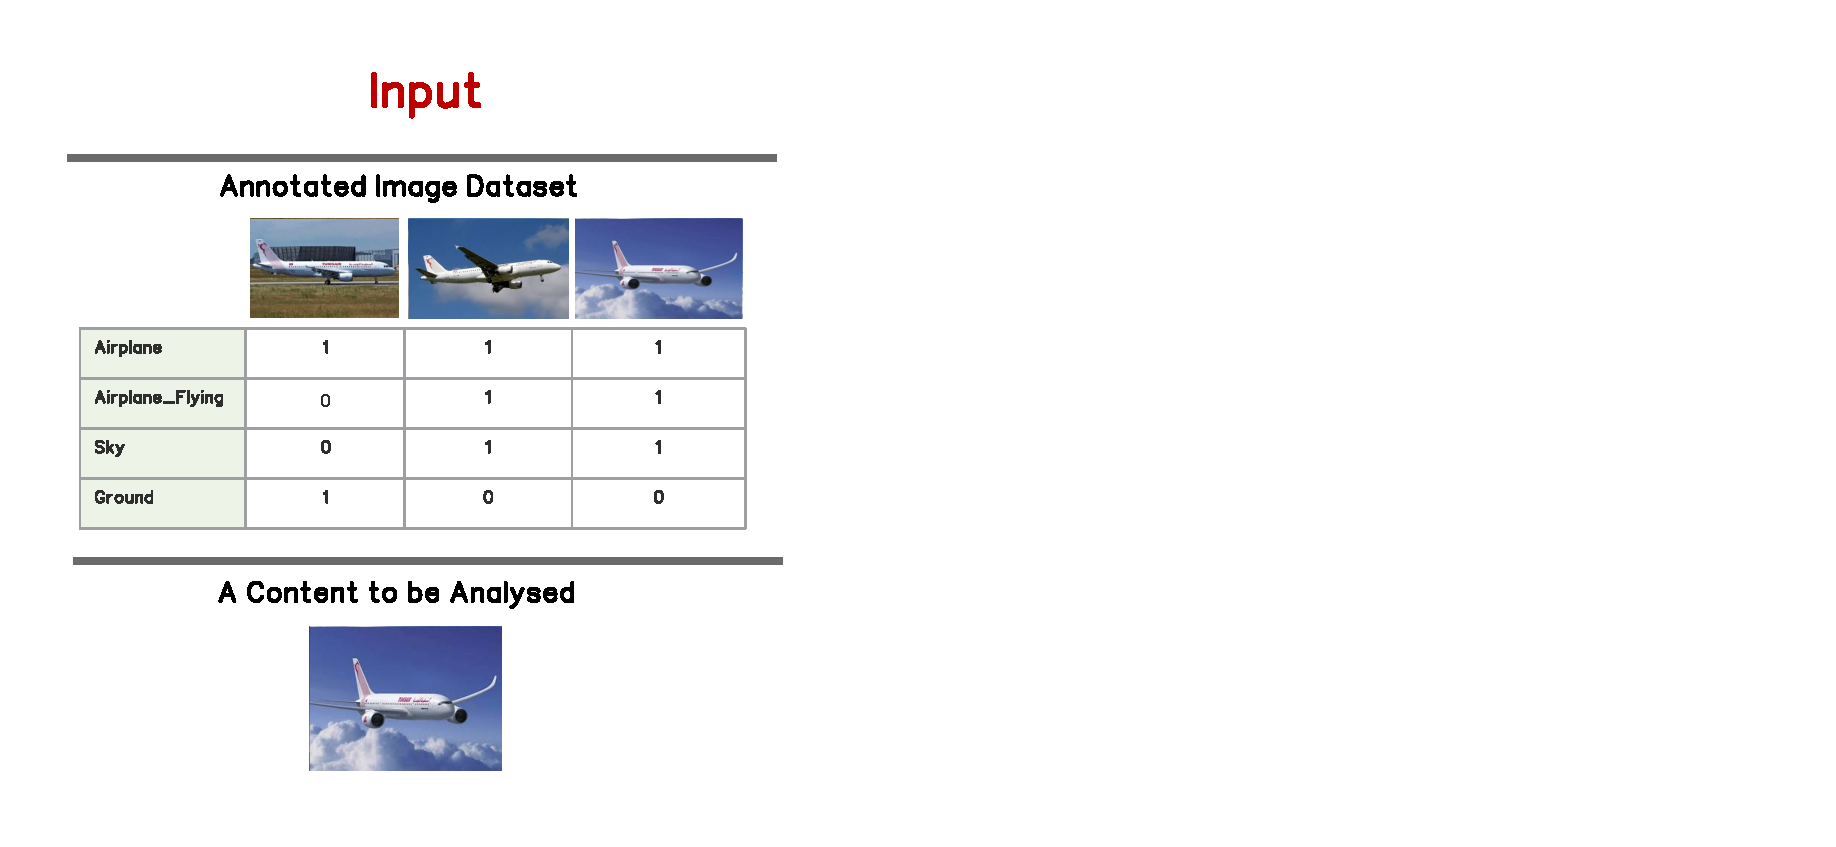
\includegraphics[scale=0.4]{graphics/c2/main_c2_1}}
\end{frame}

\begin{frame}
	\frametitle{$C_{2}$: Proposed Approach - Knowledge Extraction}
	\begin{block}{}
	 \begin{itemize}
	  \item Each \alert{concept} is considered as a Vector,
	  \item Computing \alert{similarities} between concepts for a given context.
	 \end{itemize}
	\end{block}
	{\hspace*{-1cm}\centering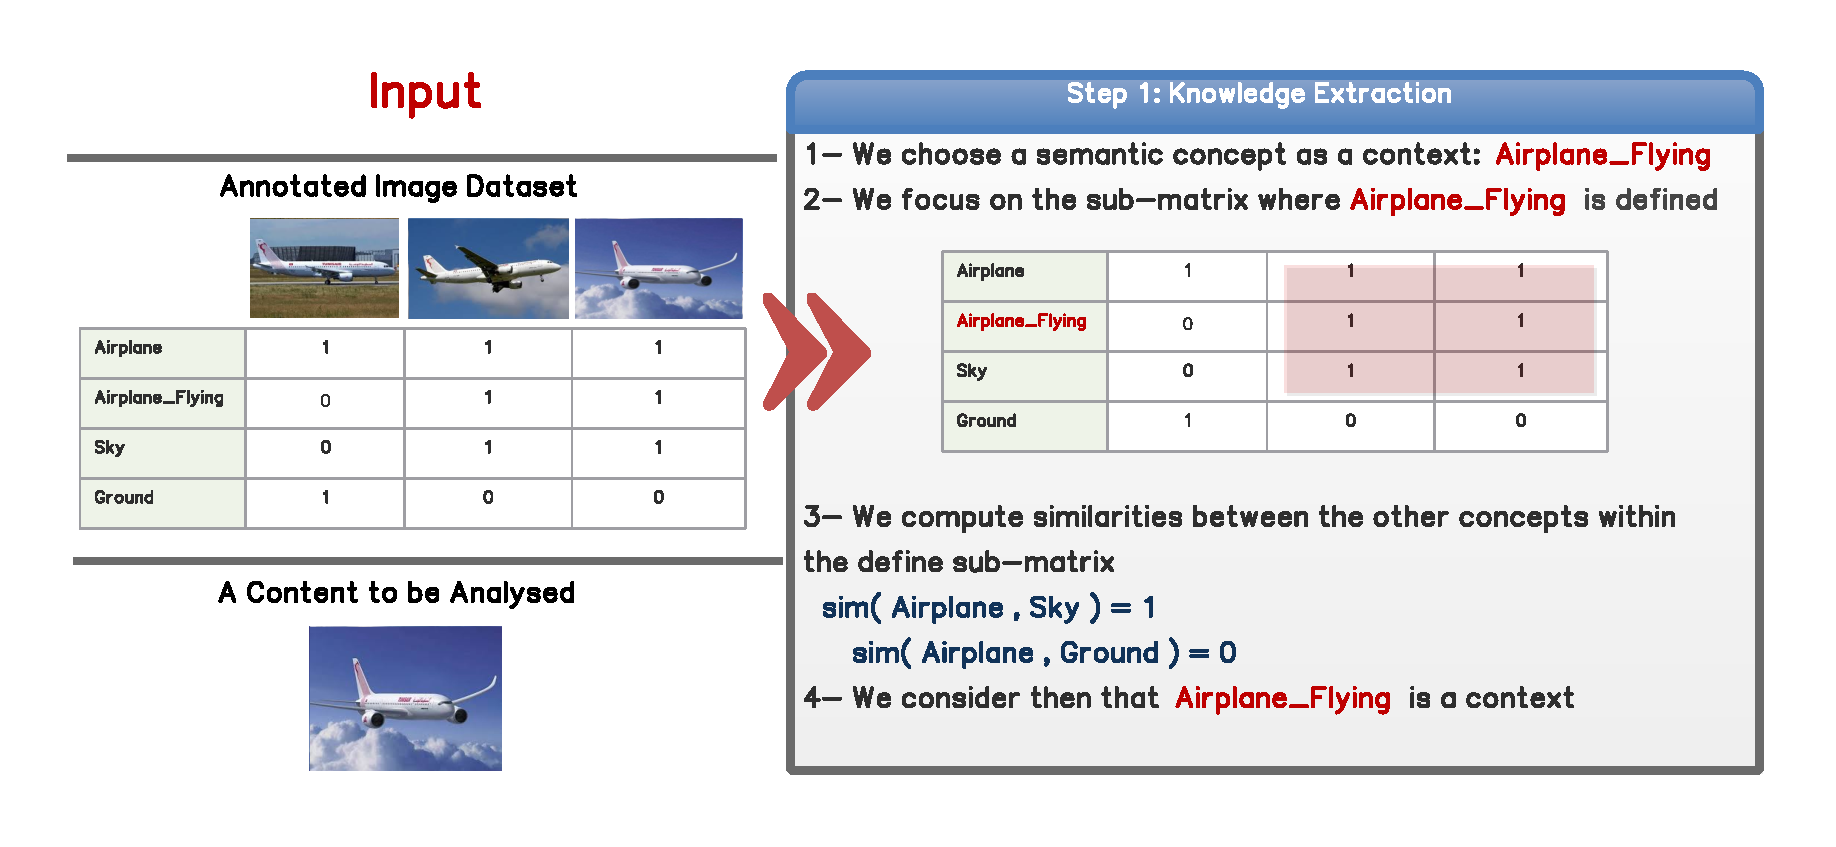
\includegraphics[scale=0.4]{graphics/c2/main_c2_2}}
\end{frame}

\begin{frame}
	\frametitle{$C_{2}$: Proposed Approach - Ontology Structure}
	\begin{block}{}
	 \begin{itemize}
	  \item \alert{Context based} ontology structure,
	  \item Computed \alert{relationships} are populated within the ontology.
	 \end{itemize}
	\end{block}
	\only<1>{\hspace*{-1cm}\centering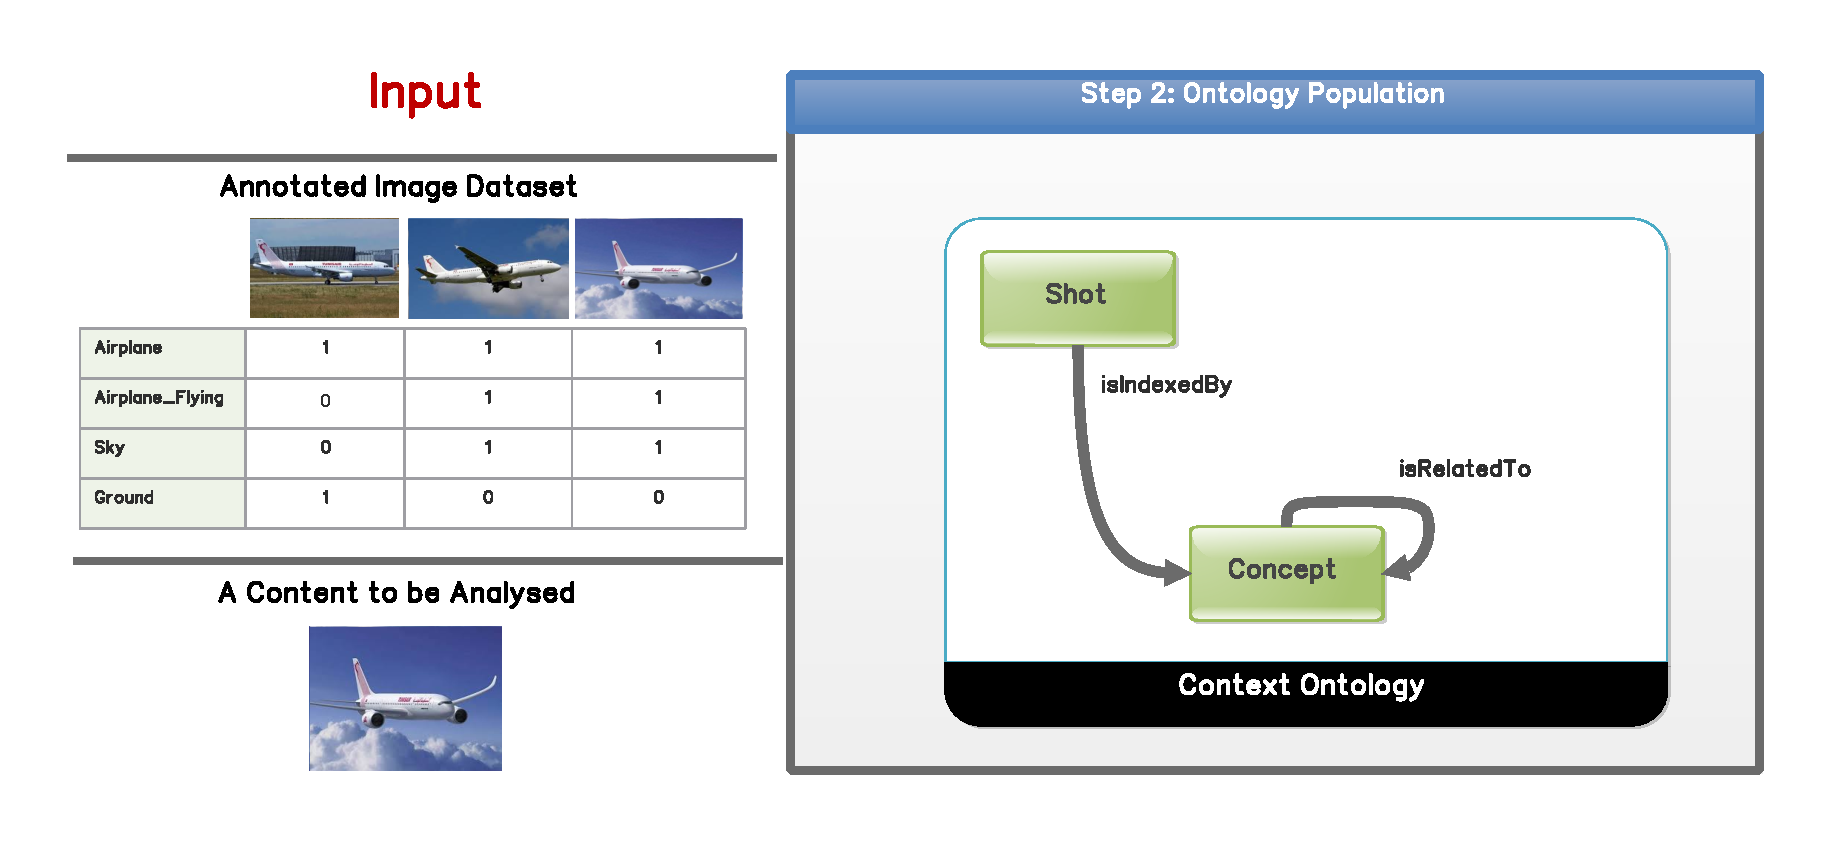
\includegraphics[scale=0.4]{graphics/c2/main_c2_3_1}}
	\only<2>{\hspace*{-1cm}\centering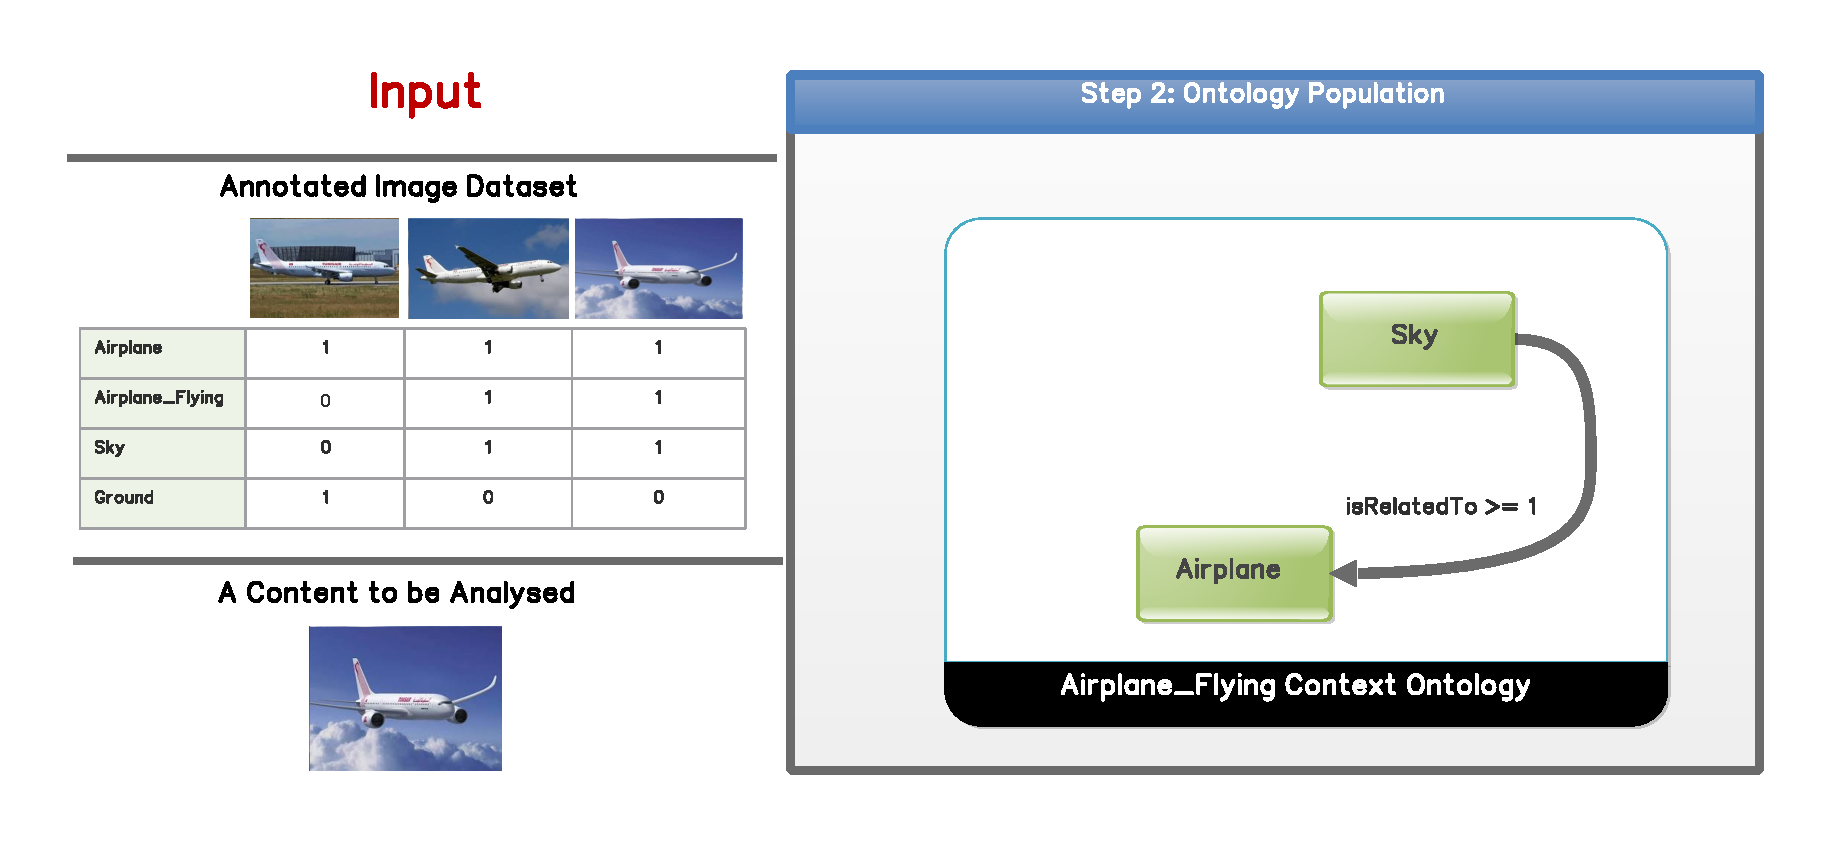
\includegraphics[scale=0.4]{graphics/c2/main_c2_3_2}}
\end{frame}

\begin{frame}
	\frametitle{$C_{2}$: Proposed Approach - Ontology Reasoning}
	\begin{block}{}
	 \begin{itemize}
	  \item Reasoning based on interpreting the \alert{$isIndexedBy$} roles,
	  \item We used \alert{\textit{``tableau''}} reasoning algorithm \tiny{\citep{Horrocks2005}}.
	 \end{itemize}
	\end{block}
	{\hspace*{-1cm}\centering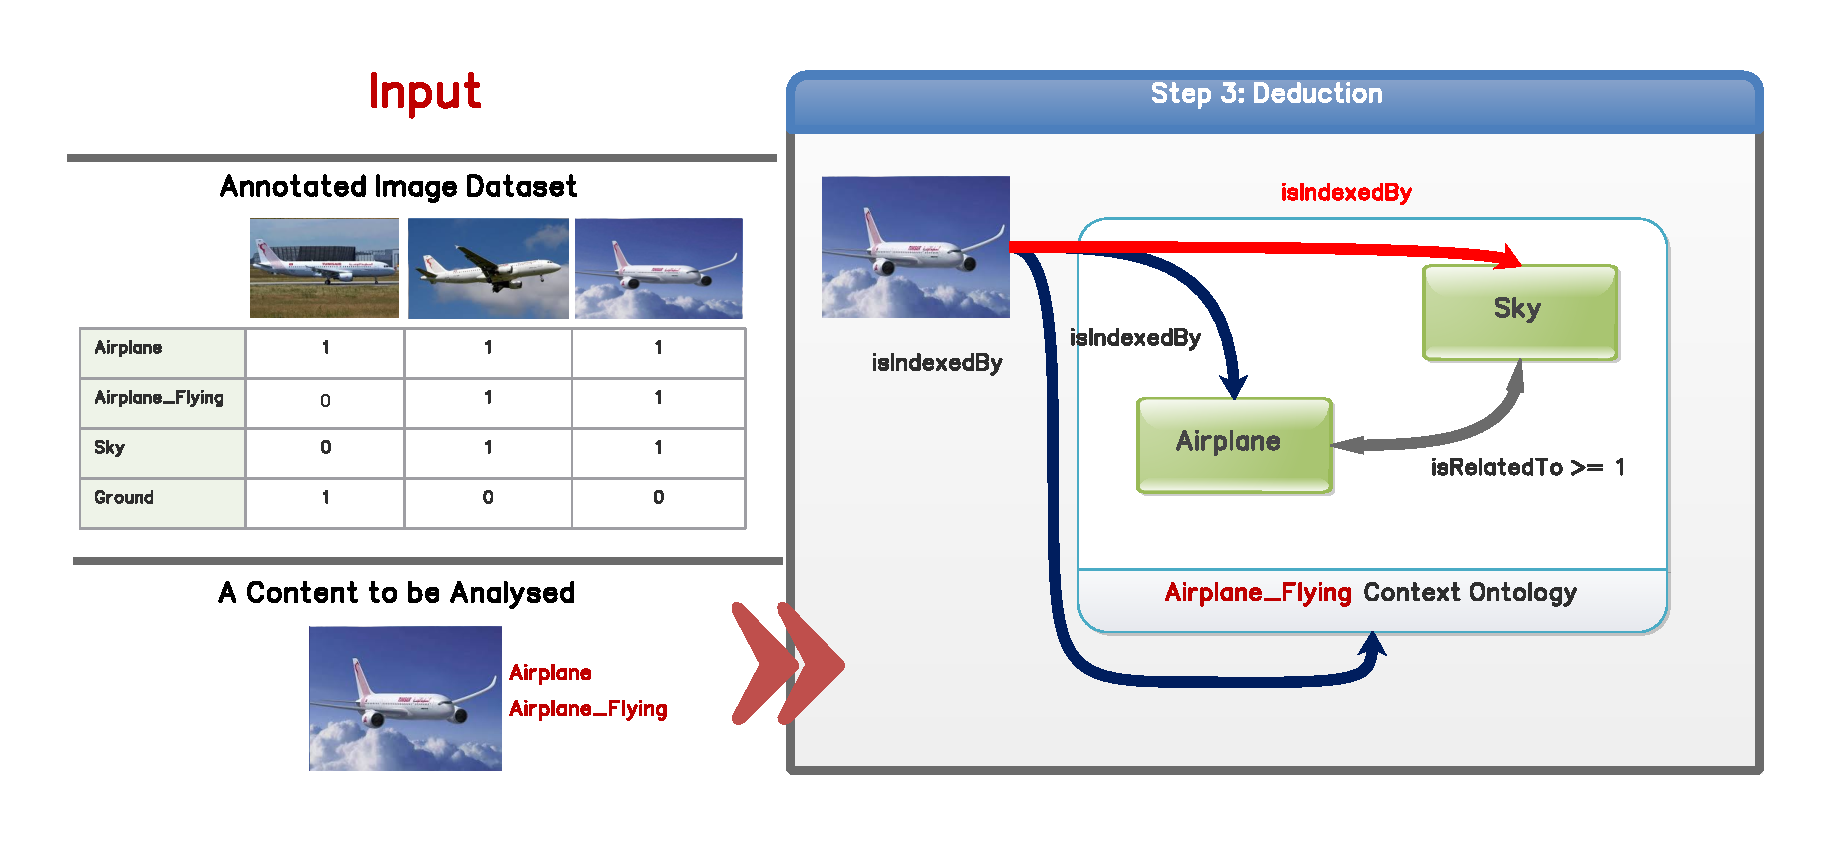
\includegraphics[scale=0.4]{graphics/c2/main_c2_4}}
\end{frame}

\begin{frame}
	\frametitle{$C_{2}$: Proposed Approach - Ontology Evolution}
	\begin{block}{}
	 \begin{itemize}
	  \item \alert{Updating} the ontology content,
	  \item The ontology evolution is based on \alert{experts} analysis.
	 \end{itemize}
	\end{block}
	{\hspace*{-1cm}\centering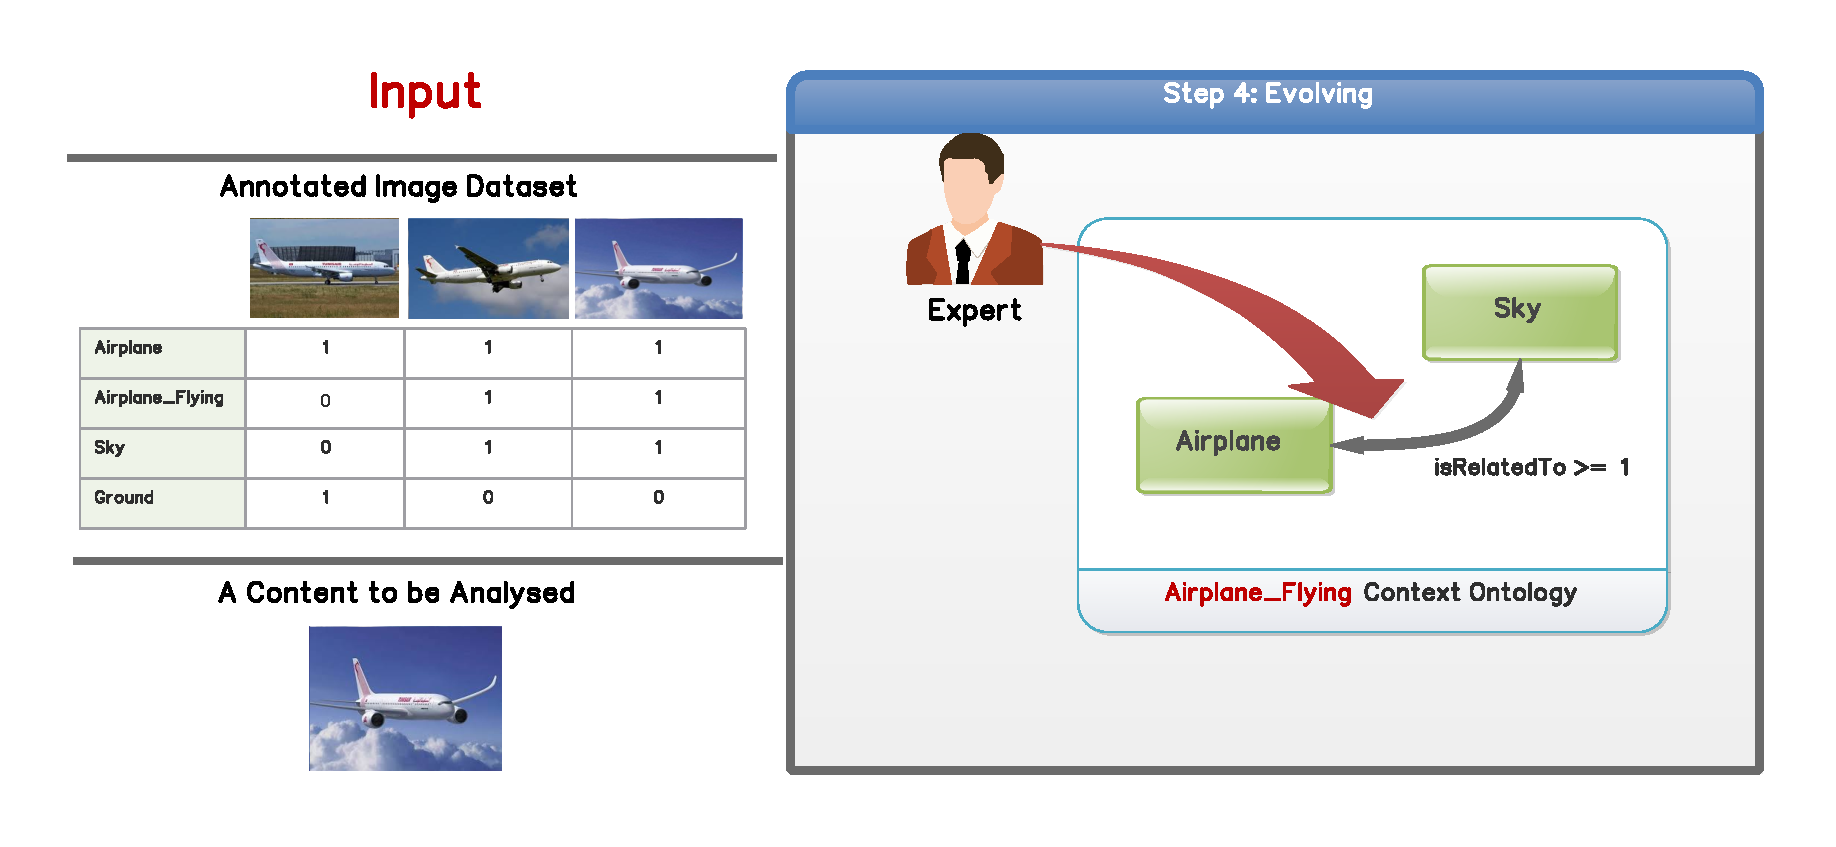
\includegraphics[scale=0.4]{graphics/c2/main_c2_5}}
\end{frame}


\begin{frame}
	\frametitle{$C_{2}$: Experiments - Setup}
	\begin{exampleblock}{Experimentation Setup}
		{\small
		\begin{itemize}		
			\item \textsc{ImageClef 2012}
			\item Photo dataset : \alert{\textbf{25.000}} images (\textbf{15.000} images for training 
				and \textbf{10.000} images for test)
			\item  \alert{94} semantic concepts
		\end{itemize}
		}
	\end{exampleblock}

	\begin{exampleblock}{Baseline}
		{\small
		\begin{itemize}
			\item We look to evaluate the semantic enhancement of a non knowledge-based approach 
			    \alert{\citep{Ksibi2012}},
			\item \alert{Visual} semantic indexing,
			\item We used the constructed \alert{contextual Ontologies}
		 \end{itemize}
		}
	\end{exampleblock}
\end{frame}

\begin{frame}
	\frametitle{$C_{2}$: Experiments - Ontologies construction}
	\begin{exampleblock}{Distribution of extracted $\mathsf{isRelatedTo}$ roles}
		 \centering \tiny
		\begin{tabular}{c l c c c c c c c c c c} \hline
		~&\textbf{Context}& $[0, 0.3[$ & $[0.3, 0.5[$ & $[0.5, 0.7[$ & $[0.7, 1.0]$ \\ 
		\hline
			1&sentiment\_euphoric	&783	&605	&510	&534\\
			2&sentiment\_happy		&2020	&864	&519	&444\\
			3&setting\_sportsrecreation&1264	&752	&483	&456\\ 
			4&age\_child		&1045	&649	&493	&441\\ 
			5&relation\_familyfriends	&1150	&903	&398	&522\\ \hline
			86&fauna\_cat	&115	&105	&91	&203\\ 
			87&fauna\_insect		&107	&63	&43	&192\\
			88&fauna\_rodent		&43	&53	&43	&139\\ 
			89&fauna\_amphibianreptile	&24	&29	&43	&127\\ 
			90&fauna\_spider	&3	&20	&16	&48\\ \hline 
			\multicolumn{2}{c}{\textbf{All contexts}}	&91803 	&50210	&27435	&33667\\
			\hline
			\multicolumn{2}{c}{\textbf{Total}}& \multicolumn{10}{c}{\textbf{\alert{203 115} $\mathsf{isRelatedTo}$ 
								roles for 90 defined contexts}}\\ \hline
		\end{tabular}
		
	\end{exampleblock}	
	%\pause
	%\begin{exampleblock}{}
	{\tiny \centering
	\begin{equation*}
			\begin{array}{ c c l c l}
			age\_adult & - &\mathcal{K}^{f}_{age\_adult} 
				& - & (age\_teenager,sentiment\_scary):\mathsf{isRelatedTo} \geq 0.12\\
			transport\_car & - &\mathcal{K}^{f}_{transport\_car}
				& - & (sentiment\_happy,timeofday\_day):\mathsf{isRelatedTo} \geq 0.95\\
			setting\_homelife & - &\mathcal{K}^{f}_{setting\_homelife} 
				& - & (quantity\_biggroup,sentiment\_happy):\mathsf{isRelatedTo} \geq 0.81\\
			\end{array}
	\end{equation*}
	}
	%\end{exampleblock}
		
\end{frame}


\begin{frame}
	\frametitle{$C_{2}$: Experiments - Obtained Results}
	\begin{exampleblock}{Enhancement Assessment}
		{\small \centering{
			\begin{tabular}{l||cc|cc} 
			
			  & \multicolumn{2}{c}{\textbf{\textit{map$_{i}$}}} 
			  &\multicolumn{2}{c}{\textbf{\textit{gmap$_{i}$}}}  \\
			  
			  & value & \% & value & \%  \\
			\hline  \hline  
		
			Our proposed framework & 
						$0,1324$ & \textbf{\alert{5.08}} & 		
						$0,0808$ & \textbf{\alert{3.46}} \\ 
			\citep{Ksibi2012}  &  $0.126$ & - & $0.078$ & -  \\
			\hline 
			\end{tabular}
		}}
	\end{exampleblock}	
	
	\begin{exampleblock}{Ontology evolution}
	{\footnotesize
		\begin{itemize}
			\item \alert{$3$} experts,
			\item Up to \alert{$0.54 \%$} of semantic enhancement.
		\end{itemize}
	}
	\end{exampleblock}
\end{frame}

\begin{frame}
	\frametitle{$C_{2}$: Related publication}
	\begin{block}{}
		\begin{itemize}
			\item \citep{Zarka2015} \textbf{Zarka, M.}, Ben Ammar, A., \&{} Alimi, A. (2016). 
				Fuzzy reasoning framework to improve semantic video interpretation. 
				\emph{Multimedia Tools and Applications}, 5719--5750.
		\end{itemize}
	\end{block}
\end{frame}

